\documentclass[9pt]{sigplanconf}

\usepackage{amssymb}
\usepackage{amsmath}
\usepackage{amsthm}
\usepackage{stmaryrd}
\usepackage{color}
\usepackage{graphics}
\usepackage{fancyvrb}
\usepackage{subfigure}
\usepackage{amsthm}
\usepackage{tikz}
\usepackage{multirow}
\usepackage{minted}

\fvset{
  linenos=true,
  fontsize=\footnotesize,
  breaklines=true,
  breakafter=+*,
  xleftmargin=\parindent
}

\usemintedstyle{vs}

\definecolor{darkblue}{rgb}{0.0,0.0,0.5}
\definecolor{darkgreen}{rgb}{0.0,0.4,0.0}
\definecolor{darkdarkgreen}{rgb}{0.0,0.35,0.0}

\newcommand{\sten}[1]{\textcolor{darkdarkgreen}{\!#1}}

\usepackage[]{hyperref}
\hypersetup{
    unicode=false,          % non-Latin characters in Acrobat's bookmarks
    pdftoolbar=true,        % show Acrobat toolbar?
    pdfmenubar=true,        % show Acrobat menu?
    pdffitwindow=false,      % page fit to window when opened
    pdftitle={},    % title
    pdfauthor={}
    pdfsubject={},   % subject of the document
    pdfnewwindow=true,      % links in new window
    pdfkeywords={keywords}, % list of keywords
    colorlinks=true,       % false: boxed links; true: colored links
    linkcolor=darkblue,          % color of internal links
    citecolor=darkblue,        % color of links to bibliography
    filecolor=green,      % color of file links
    urlcolor=blue,          % color of external links
}


\CustomVerbatimEnvironment{SpecVerbatim}{Verbatim}{fontsize=\footnotesize,xleftmargin=0.5cm,
xrightmargin=0.2cm,commandchars=\\\{\},baselinestretch=0.98,numbersep=0.9em}
\CustomVerbatimEnvironment{ExmVerbatim}{Verbatim}{fontsize=\footnotesize,xleftmargin=0.5cm,
xrightmargin=0.2cm,baselinestretch=0.98,numbers=left,numbersep=0.9em,commandchars=\\\{\}}
\CustomVerbatimEnvironment{IVerbatim}{Verbatim}{fontsize=\relsize{-1},xleftmargin=0.5cm,
xrightmargin=0.2cm,commandchars=\\\{\},baselinestretch=0.98,numbersep=0.9em}


\definecolor{darkgreen}{rgb}{0.0,0.5,0.0}
\definecolor{darkpurple}{rgb}{0.6,0.0,0.6}
\definecolor{orange}{rgb}{0.8,0.4,0.0}
\definecolor{darkorange}{rgb}{0.5,0.2,0.0}
\definecolor{marco}{rgb}{0.0,0.3,0.5}
\definecolor{gray}{rgb}{0.2,0.2,0.2}

\newcommand{\bn}{\mathbb{N}}

\newcommand{\dnote}[1]{\textcolor{darkpurple}{Dom: #1}}
\newcommand{\mnote}[1]{\textcolor{darkgreen}{Mistral: #1}}
\newcommand{\anote}[1]{\textcolor{red}{Andy: #1}}

\newcounter{block}

\newtheorem{lemma}[block]{Lemma}
\newtheorem{proposition}[block]{Proposition}
%\newtheorem{definition}[block]{Definisssstion}

\theoremstyle{definition}

\newtheorem{theorem}[block]{Theorem}
\newtheorem{remark}[block]{Remark}
\newtheorem{example}[block]{Example}
\newtheorem{definition}[block]{Definition}

% Writing macros
\newcommand{\ie}{\emph{i.e.}}
\newcommand{\eg}{\emph{e.g.}}

\newcommand{\dimId}{\texttt{dim}}

% Semantics related
\newcommand{\interp}[1]{\llbracket{#1}\rrbracket}

% Syntax macros
\newcommand{\nonterm}[1]{\textit{#1}}
\newcommand{\term}[1]{\texttt{#1}}

\newcommand{\stenRefl}[1]{\term{reflexive} \, (\term{dim=}#1)}
\newcommand{\stenFwd}[3]{\term{forward} \, (\term{depth=}#1,
  \term{dim=}#2{#3})}
\newcommand{\stenBwd}[3]{\term{backward} \, (\term{depth=}#1,
  \term{dim=}#2{#3})}
\newcommand{\stenCen}[3]{\term{centered} \, (\term{depth=}#1,
  \term{dim=}#2{#3})}
\newcommand{\irrefl}{\texttt{irreflexive}}

\newcommand{\stenReflS}[1]{\term{refl} \, (\term{dim=}#1)}
\newcommand{\stenFwdS}[2]{\term{fwd} \, (\term{depth=}#1,
  \term{dim=}#2)}
\newcommand{\stenBwdS}[2]{\term{bwd} \, (\term{depth=}#1,
  \term{dim=}#2)}
\newcommand{\stenCenS}[2]{\term{cen} \, (\term{depth=}#1,
  \term{dim=}#2)}
\newcommand{\irreflS}{\texttt{irrefl}}

% SYNTAX OPERATIONS AND PREDICATES
\newcommand{\neigh}{\textsf{neigh}}
\newcommand{\arrayTy}{\textsf{array}}
\newcommand{\rhsExp}{\textsf{rhsExp}}
\newcommand{\var}{\textsf{var}}

%% VECTOR NOTATIONS
\newcommand{\vect}[1]{\textbf{#1}}
\newcommand{\vtwoh}[2]{\setlength{\arraycolsep}{0em}
\left[\begin{array}{cc}#1 \; & \; #2\end{array}\right]}
\newcommand{\vthreeh}[3]{\setlength{\arraycolsep}{0em}
\left[\begin{array}{ccc}#1 \; & \; #2 \; & \; #3\end{array}\right]}
\newcommand{\vtwo}[2]{\setlength{\arraycolsep}{0em}
\left[\begin{array}{l}$#1$\\$#2$\end{array}\right]}
\newcommand{\vthree}[3]{\setlength{\arraycolsep}{0em}
\left[\begin{array}{l}$#1$\\$#2$\\$#3$\end{array}\right]}
\newcommand{\stwo}[4]
%{\vtwo{#1}{#2}\!\vtwo{#3}{#4}}
{\setlength{\arraycolsep}{0.1em}
\left[\begin{array}{rr}$#1$ & $#3$\\$#2$ & $#4$\end{array}\right]}

\newcommand{\singleEntry}[2]{\textbf{J}_{#2}^{#1}}
\newcommand{\zeroEntry}[2]{\textbf{K}_{#2}^{#1}}

%% OPERATIONS ON SPANS and VECTORS
\newcommand{\containedin}{\sqsubseteq}

\include{results}
\newcommand{\blasFiles}{151}
\newcommand{\blasLoC}{16046}
\newcommand{\computationalphysicstwoFiles}{16}
\newcommand{\computationalphysicstwoLoC}{793}
\newcommand{\ethreemgeaFiles}{130}
\newcommand{\ethreemgeaLoC}{45926}
\newcommand{\geoschemFiles}{576}
\newcommand{\geoschemLoC}{467207}
\newcommand{\hybridfourFiles}{29}
\newcommand{\hybridfourLoC}{4831}
\newcommand{\navierFiles}{7}
\newcommand{\navierLoC}{510}
\newcommand{\umFiles}{2552}
\newcommand{\umLoC}{625530}
\newcommand{\overallFiles}{3461}
\newcommand{\overallLoC}{1160843}


\title{Verification of Stencil Computations through Spatial Specifications}
\authorinfo{Dominic Orchard \and Mistral Contrastin
\and Matthew Danish \and Andrew Rice}{University of Cambridge}{}

\begin{document}
\maketitle

\begin{abstract}
  Verifying the correctness of numerical computations relies on first
  giving a specification of their behaviour. In many cases, a
  numerical computation is derived from an underlying mathematical
  model, but this is often difficult to use as a specification as it
  is highly decoupled from the implementation. We have been studying
  specification techniques in middle ground between low-level and
  high-level specifications for numerical code. In this paper, we
  focus on \emph{stencil computations}---a common idiom in numerical code, but
  one which is error-prone due to fine-grained indexing errors. We
  hypothesise that in practise, stencil computations tend to have a
  regular shape which is amenable to static analysis and simple
  specification. We describe a abstract specification language for
  stencil computations that can be directly embedded as annotations in
  source code, along with an inference and checking procedure. We
  evaluate our language against a corpus of numerical Fortran code,
  and show that precise specifications can be given to roughly half of
  the identifiable stencil computations, and that the vast majority of
  stencil computations indeed have a simple, regular, static
  shape. This paper details our stencil specification language, its
  static semantics, inference, checking, and program synthesis
  procedures, our implementation, and our evaluation study. We provide
  an implementation of stencil inference and validation in Camfort, an
  open-source program analysis and refactoring tool.
\end{abstract}

\keywords{program verification, specifications, static analysis,
  stencil computation}

\bibliographystyle{abbrvnat}

\section{Introduction}

\emph{Stencils} are a ubiquitous programming pattern, common in
scientific and numerical computing applications. Informally, a stencil
computation computes an array value, where the value at each index $i$ of
this array is calculated from a \emph{neighbourhood} of values around $i$ in
some input array(s), \eg{}, the Game of Life, convolutions in image
processing, approximations to differential equations. For example, the
following iteration computes the one-dimensional discrete Laplace
transform (an approximation to a derivative) in Fortran:
%
\begin{minted}{fortran}
do iter = 0, itermax
   do i = 1, (n-1)
      b(i) = a(i-1) - 2*a(i) + a(i+1)
   end do
   a = b
end do
\end{minted}
%
Line 3 is the core of the stencil computation, calculating
the value at \texttt{b(i)} from a neighbourhood of elements about
\texttt{a(i)}. Line 4 swaps
\texttt{a} and \texttt{b} between iterations, where \texttt{b} becomes the
input for the next iteration. In Fortran, parentheses \texttt{( )} are used
for array subscripts rather than the more familiar bracket syntax \texttt{[ ]}.

%This stencil computation exhibits statically decideable
%spatial and temporal relationships between $\texttt{a}$ and
%$\texttt{b}$.
In this simple example, the dependency between \texttt{a}
and \texttt{b} on line 3 forms a simple spatial relationship which is easily
understood. This spatial relationship determines other aspects of the
program and its efficient implementation: how much ``boundary'' is
needed for the array, the most cache-efficient layout in memory,
the partitioning shape for parallel implementations.

More complex stencil computations can be much harder to understand and
subsequently more prone to error. For example,
Figure~\ref{ref:navier-stokes-fragment} shows three lines from a
Navier-Stokes fluid simulator in which two arrays are read from with
different data access patterns, across two dimensions. The interaction
is much harder to understand, with the potential for the developer to
accidentally introduce an error via simple textual mistakes, for
example writing $\texttt{(i-1,j)}$ instead of $\texttt{(i+1,j)}$.

In this work, we introduce a simple specification language for the
spatial properties of stencil computations. The
specifications abstract over the fine grained detail of stencil access
patterns. In practice, most stencil computations have a regular shape
that can be described simply and abstractly, with a small set of
coarse-grained descriptions. In the case of our first Laplace example,
our inference procedure provides the specification:
%
\begin{minted}{fortran}
!=  stencil centered(depth=1, dim=1) :: a
\end{minted}
%
This explains that \texttt{a} is read from with a
symmetrical stencil pattern (``centered'') to a depth of one in each
direction in its first (and only) dimension.
%The second line explains
%the temporal relationship between \texttt{b} and \texttt{a}: that
%previous time step for \texttt{b} is actually provided by \texttt{a},
%and vice versa. This is explained as a mutual dependence between
%\texttt{a} and \texttt{b}.
In the case of the Navier-Stokes example of
Figure~\ref{ref:navier-stokes-fragment}, its inferred specification is shown
in Figure~\ref{ref:navier-stokes-fragment}(b). The
specification explains that, over the whole fragment, \texttt{u} is
read from with a centered pattern to depth of 1 in both dimensions
(this is known as the \emph{five point stencil}) and \texttt{v}
is read from in a neighbourhood bounded by forward to depth of $1$ in
the first dimension and backward to a depth of $1$ in the second
dimension. Figure~\ref{ref:navier-stokes-fragment}(c) describes these
pictorially.

In this paper, we make the following contributions:
%
\begin{itemize}
\item we introduce a specification language for
stencil computations that captures many common forms
of data access pattern, both spatial and temporal (Section~\ref{sec:lang});
\item we detail inference and checking
algorithms for stencil specifications (Section~\ref{sec:analysis});
\item we evaluate our implementation of the approach
in the CamFort tool for Fortran verification, studying
a number of example programs to assess the usefulness
of this approach.
\dnote{insert results here}
\end{itemize}
%

\begin{figure}[t]
  \begin{minted}[firstnumber=20]{fortran}
du2dx = ((u(i,j)+u(i+1,j))*(u(i,j)+u(i+1,j))+ &
  gamma*abs(u(i,j)+u(i+1,j))*(u(i,j)-u(i+1,j))- &
  (u(i-1,j)+u(i,j))*(u(i-1,j)+u(i,j))- &
  gamma*abs(u(i-1,j)+u(i,j))*(u(i-1,j)-u(i,j))) &
  /(4.0*delx)

duvdy = ((v(i,j)+v(i+1,j))*(u(i,j)+u(i,j+1))+ &
  gamma*abs(v(i,j)+v(i+1,j))*(u(i,j)-u(i,j+1))- &
  (v(i,j-1)+v(i+1,j-1))*(u(i,j-1)+u(i,j))- &
  gamma*abs(v(i,j-1)+v(i+1,j-1))*(u(i,j-1)-u(i,j))) &
  /(4.0*dely)

laplu = (u(i+1,j)-2.0*u(i,j)+u(i-1,j))/delx/delx+ &
  (u(i,j+1)-2.0*u(i,j)+u(i,j-1))/dely/dely
\end{minted}
(a) Excerpt from Fortran code for a Navier-Stoke fluid simulator,
showing highly-detailed stencil computations. \\

%\begin{SpecVerbatim}[xleftmargin=0.1cm]
%20-24  u: centered depth=1 dim=1
%6-30  u: centered depth=1 dim=2
%      v: forward depth=1 dim=1, backward depth=1 dim=1
%32-33  u: centered depth=1 dim=1,2
%\end{SpecVerbatim}

\begin{minted}{fortran}
!= stencil centered(depth=1,dim=1)*reflexive(dim=2) + centered(depth=1,dim=2)*reflexive(dim=1) :: u

!= stencil forward(depth=1,dim=1) * backward(depth=1,dim=2) :: v
\end{minted}
(b) Inferred stencil specification from CamFort

\begin{center}
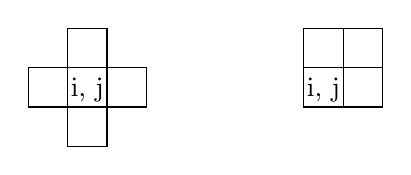
\begin{tikzpicture}
\node at (1.25,1.22) {i, j};
\draw (1,1) rectangle (1.5,1.5);
\draw (1.5,1) rectangle (2,1.5);
\draw (1,0.5) rectangle (1.5,1);
\draw (0.5,1) rectangle (1,1.5);
\draw (1,1.5) rectangle (1.5,2);
%
\node at (4.25,1.22) {i, j};
\draw (4,1) rectangle (4.5,1.5);
\draw (4.5,1) rectangle (5,1.5);
\draw (4.5,1.5) rectangle (5,2);
\draw (4,1.5) rectangle (4.5,2);
\end{tikzpicture}
\end{center}
(c) Pictorial representation of the two stencil specifications.
The horizontal dimensions is \text{dim=1} and the vertical is \texttt{dim=2}:
\caption{Fragment of Navier-Stokes fluid simulator and its specification}
\label{ref:navier-stokes-fragment}
\end{figure}

\section{Stencil specification language}
\label{sec:lang}

Our specification system is based on the observation
that most forms of array access in numerical code have
a fixed, statically-determined access pattern. For example, the
``\emph{five-point stencil}'' on a two-dimensional array reads from array
indices $(i, j)$, $(i-1, j)$, $(i+1, j)$, $(i, j-1)$, and $(i, j+1)$
for all $i, j$ within the inner boundary of the array (to avoid
out-of-bounds access at the edges). We revisit this hypothesis
in Section~\ref{sec:evaluation} where the inference of
such regular stencil patterns on a corpus of numerical programs (both
small and large). We found that indeed \dnote{..}.

We outline the specification language here. Section~\ref{sec:syntax}
outlines the syntax. Section~\ref{sec:semantics} defines its semantics
via a simple set interpretation over indices. Section~\ref{sec:eqs} provides an
equational theory for specifications via relation ($\equiv$) and a
theory of approximation via relation ($<:$). These equations are then
proven sound with respect to the set semantics of Section~\ref{sec:semantics}.

\subsection{Notation and convention}
\label{sec:notation}

\renewcommand*{\arraystretch}{0.8}
\paragraph{Target language syntax} Throughout, for the source language
syntax, $v$ ranges over program variables, $s$ over statements, and
$e$ over expressions (which may be impure).  By ``variable'', we mean
in the imperative sense (\ie{}, named binders to memory cells) instead
of mathematical variables. We make clear a number of standard notions
used throughout.

\begin{definition}[Base induction variable]
  A variable \textit{v} of integer type is a \emph{base induction
    variable} if it is the control variable of a ``for''
  loop\footnote{Or equivalent for the target language, \eg{},
    \texttt{do} in Fortran for our implementation}, incremented by $1$ per
iteration. The variable is marked as a base induction variable
only within the scope of the loop, and such variables will be ranged
over by $i$, $j$, $k$. Since we do not use non-base induction
variables (which are traditionally affine transformations of induction
variables) we often simply say \emph{induction variable}.
\end{definition}

\begin{definition}[Array subscript]
  An \emph{array subscript} is an expression that indexes an array
  (for the purpose or reading or writing an element), which we denote
  by $v(\bar{e})$ for the source language where $\bar{e}$ is shorthand
  for a syntactic list of indexing expressions. A \emph{relative
    index} is a list $\bar{e}$ where each $e \in \bar{e}$ is defined
  in terms of some base induction variable.
\end{definition}

\begin{definition}[Neighbourhood index and neighbourhood subscripts]
  For an array subscript $v(\bar{e})$, we say that $e \in \bar{e}$
  is a \emph{neighbourhood index} if it is of the form
  $e \equiv i$, $e \equiv i + a$ or $e \equiv i - a$ where $a$ is a
  constant of integer type. That is, a neighbourhood index is a
  relative index defined as a constant translation of a base induction
  variable. The relation $\equiv$ identifies terms up-to commutativity
  of $+$ and the inverse relation of $+$ and $-$ (\eg{},
  $(-b) + i \equiv i - b$).  We classify neighbourhood indices using
  the predicate \neigh{}. An array subscript $v(\bar{e})$ where every
 $e \in \bar{e}$ is a neighbourhood index is called a
 \emph{neighbourhood subscript}.
\end{definition}


\subsection{Specification syntax}
\label{sec:syntax}

Figure~\ref{fig:syntax} gives the syntax of stencil specifications,
which we introduces in stages below.  The top-level is given by the
\nonterm{specification} production which splits into either a
\nonterm{regionDec} (region declaration) or a \nonterm{specDec}
(specification declaration). Specification declarations associate a
specification to one or more program variables $\bar{v}$ (here given
using the Fortran style syntax of $\ldots \; \texttt{::} \bar{v}$),
describing how the array variables $\bar{v}$ are accessed.
%Specification declarations are either \nonterm{spatial} or
%\nonterm{temporal} specifications and describe, for spatial
%specifications,
%Specifications declarations describe
%how an array variable $v$ is read
%, and for temporal
%specifications what variables are used to define the array variable $v$.
%%

%\subsubsection{Spatial specification syntax}

\emph{Regions} are the central building blocks of spatial
specifications. Regions can either be declared along with a
\nonterm{regionDec}, assigning a region specification \nonterm{region} to
a region variable \nonterm{rvar} or given directly within a
\nonterm{spatial} specification.

\paragraph{Region constants}

Regions have as terminals the \emph{region constants}, denoted by
\term{reflexive}, \term{forward}, \term{backward}, or \term{centered}. Each
region constant except \term{reflexive} is given a depth parameter $n$ (natural
number greater than 0). They all receive a dimension identifier $d$ (also a
natural number greater than 0). Region constants specify that an array is read
from by a collection of indices which in the $d^{th}$ dimension are
neighbourhood indices ranging from $i + 0$ up to $i \pm n$ inclusively,
\eg{}, the following is valid stencil, reading from \term{a} and writing to
\term{b}:
%%
\begin{minted}{fortran}
!= stencil forward(depth=2, dim=1) :: a
b(i, 0) = a(i, 0) + a(i+1, 0) + a(i+2, 0)
\end{minted}
%%
were \texttt{i} is an induction variable.  The stencil specification
is associated to the array variable \texttt{a}. Note that the second
dimension is fixed at a constant here.

A \term{backward} stencil
is similar but has negative neighbourhood indices, \eg{},
%
\begin{minted}{fortran}
!= stencil backward(depth=2, dim=1) :: a
b(i) = a(i) + a(i-1) + a(i-2)
\end{minted}
%
A \texttt{centered} stencil is a combination of \texttt{forward}
and \texttt{backward} stencils to the same depth, \eg{},
%%
\begin{minted}{fortran}
!= stencil centered(depth=1, dim=1) :: a
b(i) = ( a(i) + a(i-1) + a(i+1) ) / 3.0
\end{minted}

\begin{figure}[t]
\begin{align*}
\def\arraystretch{1.2}
\setlength{\arraycolsep}{0.2em}
\newcommand{\dimTy}{\mathbb{D}}
\begin{array}{rl}
\nonterm{specification} ::= & \nonterm{regionDec} \mid \nonterm{specDec} \\
\nonterm{specDec} ::= & \term{stencil} \; \nonterm{specTop} \;
                        \texttt{::} \; v
  \\
\nonterm{regionDec} ::= &  \texttt{region} \; \nonterm{rvar} \; \texttt{=} \;
                         \nonterm{region}\\[1em]
%\nonterm{spec} ::= & \nonterm{spatial} \mid \nonterm{temporal}
%\\[1em]
\nonterm{specTop} ::= & [\nonterm{approxMod},] \; \nonterm{spec} \\
\nonterm{spec} ::= & [\nonterm{multMod},] \; \nonterm{region} \\
\nonterm{multMod} ::= & \term{readOnce} \\
\nonterm{approxMod} ::= & \term{atMost} \; \mid \; \term{atLeast} \\[0.1em]
\nonterm{region} ::= 
        & \stenFwd{\mathbb{N}_{>0}}{\dimTy}{\;[, \texttt{irreflexive}]} \\
\mid \; & \stenBwd{\mathbb{N}_{>0}}{\dimTy}{\;[, \texttt{irreflexive}]} \\
\mid \; & \stenCen{\mathbb{N}_{>0}}{\dimTy}{\;[, \texttt{irreflexive}]} \\
\mid \; & \stenRefl{\dimTy}  \\
\mid \; & \nonterm{region} \; \term{+} \; \nonterm{region} \\
\mid \; & \nonterm{region} \; \term{*} \; \nonterm{region} \\
\mid \; & \nonterm{rvar}  \\[0.5em]
%\nonterm{temporal} ::= \; & \term{dependency} \; (v \; \{ , v \}) [, \texttt{mutual}]
%  \\[0.5em]
\dimTy ::= \; & \mathbb{N}_{>0} \\
\nonterm{rvar} ::= \; & [\text{\term{a}-\term{z}$\,$\term{A}-\term{Z}$\,$\term{0}-\term{9}}]+
\end{array}
\end{align*}
\caption{Specification syntax (EBNF grammar)}
\label{fig:syntax}
\end{figure}

\paragraph{Sum and product of regions}
%%
Region terms can be combined using the sum operator
\term{+} or the product operator \term{*}.

The sum of two regions $r \texttt{+} r'$ specifies that an array is
read using the neighbourhood indices described by either $r$ or
$r'$. It can be thought of as a disjunction of specifications. For
example, the following gives the specification for the five-point
stencil which is the sum of two compound \texttt{reflexive} and
\texttt{centered} regions in each dimension:
%%
\begin{minted}{fortran}
!= stencil centered(depth=1, dim=1)*reflexive(dim=2) + centered(depth=1, dim=2)*reflexive(dim=1) :: a

b(i,j) = -4*a(i,j) + a(i-1,j) + a(i+1,j)
                   + a(i,j-1) + a(i,j+1)
\end{minted}
%%
Here the left hand side of \texttt{+} says when the second dimension
(induction variable $j$) is fixed at the origin, the first dimension
(induction variable $i$) accesses immediate vicinity of the origin.
The right hand side of \texttt{+} is similar but the dimensions are reversed.
This reflects the symmetry under rotation in the fivepoint stencil.

The product of two regions $r \texttt{*} r'$ specifies that the array
is read with neighbourhood indices drawn from the bounding box created
by the regions two regions $r$ and $r'$. For example, the following
code (defining a nine-point stencil) has a specification as the
product of two \texttt{centered} regions in each dimension:
%%
\begin{minted}[breakindent=2.9em]{fortran}
x = a(i, j)   + a(i-1, j)   + a(i+1, j)
y = a(i, j-1) + a(i-1, j-1) + a(i+1, j-1)
z = a(i, j+1) + a(i-1, j+1) + a(i+1, j+1)

!= stencil centered(depth=1, dim=1) * centered(depth=1, dim=2) :: a
b(i, j) = (x + y + z) / 9.0
\end{minted}
%%
Such a stencil computation is a common image convolution (for example
for edge detection).
Note that there are a number of intermediate assignments over which
the whole specification ranges.

The region constructor \texttt{*} can also be interpreted as conjunction of
two specifications since they need to hold simultaneously for their
corresponding dimensions.

As another example, the following code and specification
implements the \emph{Roberts cross}
edge-detection convolution~\cite{davis1975survey}:
%%
\begin{minted}[breakindent=5.5em]{fortran}
do j=0, jmax-1
    do i=0, imax-1
      x = a(i,j) - a(i+1,j+1)
      y = a(i+1,j) - a(i,j+1)
      != stencil forward(depth=1,dim=1) * forward(depth=1,dim=2) :: a
      b(i,j) = sqrt(x*x+y*y)
   end do
end do
\end{minted}

\paragraph{Region declarations and variables}

Region specifications can be assigned to region variables via
a region declaration, which can be used later to form a spatial
specification. For example, the specification from the previous
 example can be restated as:
%%
\begin{minted}{fortran}
!= region r1 = centered(depth=1, dim=1)
!= region r2 = centered(depth=1, dim=2)
!= region robertsCross = r1*r2
!= stencil robertsCross :: a
\end{minted}
This is especially useful for common stencils such as Robert's cross
as the region can be defined once and used by region name many times.
%%
\paragraph{Spatial modifiers}
%%
There are two modifiers one used at specification the other at region
level to provide better descriptions for stencil computations.

At the specification level, the \texttt{readOnce} modifier enforces that no 
index appears more than once. For example, in all of the previous examples the
\texttt{readOnce} modifier could be added, \eg{}
%
\begin{minted}{fortran}
!= stencil readOnce, backward(depth=2, dim=1) :: a
b(i+1) = a(i) + a(i-1) + a(i-2)
\end{minted}
%
However, this would be an invalid specification if any of the
array subscripts was repeated. This modifier provides a way to
rule out any accidental repetition of array subscripts.
The notion corresponds to that of \emph{linearity} in type systems,
though we opt for the more informative and easily understood name
\texttt{readOnce}. This modifier is optional, so it need not
be present even if the stencil is linear.

At the region level, \texttt{irreflexive} modifier qualifies base
regions of \texttt{forward}, \texttt{backward}, and \texttt{centered}.
It indicates that in the dimension of the region there is no neighbour index
with $0$ offset, \eg{},
%
\begin{minted}{fortran}
!= stencil centered(depth=1, dim=1, irreflexive) :: a
b(i) = a(i+1) + a(i-1)
\end{minted}
%
or with just a \texttt{forward} region an example would be:
%
\begin{minted}{fortran}
!= stencil forward(depth=1, dim=1, irreflexive) :: a
b(i) = a(i+1)
\end{minted}

Naturally, \term{irreflexive} qualifier cannot be used on \term{reflexive}
regions.

\paragraph{Under and over-approximation}

In some cases, it is useful to give a lower and/or upper bound for a
stencil. This can be done using either the \term{atMost} or
\term{atLeast} modifiers. This is particularly useful in situations
where there is a non-contiguous stencil, which does not fit the rest
of the specification syntax. For example:
%%
\begin{minted}{fortran}
!= stencil atLeast, reflexive(dim=1)      :: a
!= stencil atMost, forward(depth=2, dim=1) :: a
b(i) = a(i) + a(i+2)
\end{minted}
%%
%\subsubsection{Temporal specifications}


\subsection{Note on the design}

The names ``forward'', ``backward'' and ``centered''
are inspired by standard terminology in numerical analysis
for the shape of discretisation schemes. For example,
the standard ``explicit method'' for approximation
PDEs is the \emph{Forward Time, Centered Space} (FTCS)
scheme~\cite{dawson1991finite}. For
the one-dimensional heat equations, an FTCS discretisation
provides approximation code with the following stencil~\cite{recktenwald2004finite}:
%%
\begin{minted}{fortran}
do i=2, n-1
  u(i) = r*v(i-1) + r2*v(i) + r*v(i+1)
end do
\end{minted}
%%
where \texttt{r} and \texttt{r2} are some constants.
A valid specification for this stencil is then:
%%
\begin{minted}{fortran}
!= stencil centered(depth=1, dim=1) :: v
\end{minted}
%%
Such a specification can be inferred, or can be inserted by a user
and checked against the code.

\subsection{Equational theory and approximations}
\label{sec:eqs}

\begin{figure}
\begin{align*}
\setlength{\arraycolsep}{0.05em}
\begin{array}{c}
\framebox{$\textit{region} \equiv \textit{region}'$} \\[1em]
\begin{array}{rll}
(\textsc{F\; \texttt{+} \;F}) \;\; &
\stenFwdS{n \, \textsf{max} \, m}{d} \\
 \equiv \; & \stenFwdS{n}{d} \; \texttt{+} \; \stenFwdS{m}{d} \\[1em]
%
(\textsc{B\; \texttt{+} \;B}) \;\; &
\stenBwdS{n \, \textsf{max} \, m}{d} \\
 \equiv \; & \stenBwdS{n}{d} \; \texttt{+} \; \stenBwdS{m}{d} \\[1em]
%
(\textsc{C\; \texttt{+} \;C}) \;\; &
\stenCenS{n \, \textsf{max} \, m}{d} \\
\equiv \; & \stenCenS{n}{d} \; \texttt{+} \; \stenCenS{m}{d} \\[1em]
%
(\textsc{C\; \texttt{+} \;F}) \;\; & \stenCenS{n}{d} \\
\textit{$m \leq n$} \; \equiv \; & \stenCenS{n}{d} \; \texttt{+} \;
                      \stenFwdS{m}{d} \\[1em]
%
(\textsc{C\; \texttt{+} \;B}) \;\; &
\stenCenS{n}{d} \\
\textit{$m \leq n$} \; \equiv \; & \stenCenS{n}{d} \; \texttt{+} \;
                      \stenBwdS{m}{d} \\[1em]
(\textsc{B\; \texttt{+} \;F}) \;\; &
\stenCenS{n}{d} \\
\equiv \; & \stenFwdS{n}{d} \; \texttt{+} \; \stenBwdS{n}{d} \\[1em]
(\textsc{R \; \texttt{+} \; F}) \;\; &
\stenFwdS{n}{d} \\
\equiv \; & \stenReflS{d} \; \texttt{+} \; stenFwdS{n}{d} \\[1em]
%
%
%
(\texttt{+}\textsc{idem}) \;\; & S \; \texttt{+} \; S \; \equiv \; S \\[0.5em]
%
(\texttt{+}\textsc{comm}) \;\; & S \; \texttt{+} \; T \; \equiv \; T \;
                       \texttt{+} \; S \\[0.5em]
%
(\texttt{+}\textsc{assoc}) \;\; & R \; \texttt{+} \; (S \; \texttt{+} \; T) \; \equiv \; (R \;
                       \texttt{+} \; S) \; \texttt{+} \; T \\[0.5em]
(\texttt{*}\textsc{comm}) \;\; & S \; \texttt{*} \; T \; \equiv \; T \;
                       \texttt{*} \; S \\[0.5em]
%
(\texttt{*}\textsc{assoc}) \;\; & R \; \texttt{*} \; (S \; \texttt{*} \; T) \; \equiv \; (R \;
                       \texttt{*} \; S) \; \texttt{*} \; T \\[0.5em]
(\textsc{dist}) \;\; & R \; \texttt{*} \; (S \; \texttt{+} \; T) \; \equiv \; (R \;
                       \texttt{*} \; S) \; \texttt{+} \; (R
                       \; \texttt{*} \; T) \\[0.5em]
\end{array} \\ \\
%
\framebox{${\textit{specDec} :: \texttt{v}} \equiv
{\textit{specDec'} :: \texttt{v}}$} \\[1em]
\begin{array}{rl}
% MUTUAL
%(\textsc{mutual}) \; &
%\texttt{stencil} \; \texttt{dependency} (\texttt{v}), \texttt{mutual}
%  :: \texttt{w}
%\\
%\equiv \; & \texttt{stencil} \; \texttt{dependency} (\texttt{w}), \texttt{mutual} ::
%  \texttt{v} \\[0.5em]
%(\textsc{coalesce}) \; &
%\texttt{stencil} \; \texttt{dependency} (\bar{v})
%  :: \texttt{v} \\
%& ; \texttt{stencil} \; \texttt{dependency} (\bar{w})
%  :: \texttt{v}
%\\
%\equiv \; & \texttt{stencil} \; \texttt{dependency} (\bar{v}, \bar{w}) ::
%  \texttt{v} \\[0.5em]
(\textsc{spatial}) \; &
(\textit{region} \equiv \textit{region'}) \\
\Rightarrow \; & (\texttt{stencil} \; [\textit{mod}] \; [\textit{approxMod},] \;
\textit{region} \\
& \!\!\equiv \; \texttt{stencil} \; [\textit{mod}] \;
            [\textit{approxMod},] \;
\textit{region}') \\
\end{array}
\end{array}
\end{align*}
\caption{Equations on specifications}
\label{fig:equations}
\end{figure}


\paragraph{Equations}
Figure~\ref{fig:equations} lists the equational theory for
specifications. This is broken down into equations on regions only,
given by the equivalence relation $\textit{region} \equiv \textit{region}'$ and
on specification declarations assigned to variables via the equivalence relation
$\textit{specDec} :: \texttt{v} \equiv
\textit{specDec'} :: \texttt{v}$.

To save space we use abbreviations
\term{refl}, \term{fwd}, \term{bwd}, and \term{cen} for \term{reflexive},
\term{forward}, \term{backward}, and \term{centered} regions respectively.
The equations reveal something of their semantics.  The first six
equations (with labels of the form $\ldots \texttt{+} \ldots$)
explain the behaviour of overlapping regions with sum
\term{+}. The next six equations explain the algebraic behaviour of
\term{+} and \term{*}.  Together, we see that \term{+} is an
associative, commutative, idempotent binary operator that distributes
with \term{*}, which is associative and commutative. This distribution
of \term{*} over \term{+} is key as it is used internally to give a
normal form for stencil specifications akin to Disjunctive Normal Form
(DNF) (where \term{+} is taken as ``disjunction'' and \term{*} as the
``conjunction''). We revisit this normalisation in Section~\ref{}.

\begin{figure}[t]
\begin{align*}
\begin{array}{c}
\dfrac{}{S <: S}(\textsc{refl}) \qquad \dfrac{R <: S \quad S <: T}{R <:
  T}(\textsc{trans}) \\[1.5em]
\dfrac{}{\texttt{readOnce} \, S <: S}(\textsc{rep})
\\[1.5em]
\setlength{\arraycolsep}{0.1em}
\dfrac{\hspace{3em} m \leq n \hspace{3em}}
{\begin{array}{rl}
\stenFwdS{m}{d} & <: \stenFwdS{n}{d}
%& \;\, ds \subseteq es \wedge n \leq m
\\
\wedge \stenBwdS{m}{d} & <: \stenBwdS{n}{d}
%& \;\, ds \subseteq es \wedge n \leq m
\\
\wedge \; \stenCenS{m}{d} & <: \stenCenS{n}{d}
%& \;\, ds \subseteq es \wedge n \leq m
\\
\wedge \; \stenBwdS{m}{d} & <: \stenCenS{n}{d} \\
\wedge \; \stenFwdS{m}{d} & <: \stenCenS{n}{d} \\[1em]
\end{array}} \\[2.5em]
\hspace{-0.5em}
\dfrac{S_1 <: T_1 \quad S_2 <: T_2}
      {S_1 \, \texttt{+} \, S_2 <: T_1 \, \texttt{+} \, T_2}
(\textsc{cong}\texttt{+}) \;\;\;
\dfrac{S_1 <: T_1 \quad S_2 <: T_2}
      {S_1 \, \texttt{*} \, S_2 <: T_1 \, \texttt{*} \, T_2}
(\textsc{cong}\texttt{*})
\end{array}
\end{align*}
\caption{Inequations on regions}
\label{fig:inequations}
\end{figure}

\paragraph{Inequations: sub-specifications}

Figure~\ref{fig:inequations}

\section{Semantics of specifications; a model}
\label{sec:semantics}

\newcommand{\relix}{(\mathbb{Z}_\bot)^\mathbb{D}}

We provide a semantic model of the stencil specification language as
the basis for building correct implementations, showing the soundness
of the equational theory and approximations, and as a basis for the
inference, checking, and program synthesis algorithms.
The semantics of stencil specifications can be given a denotational
model as sets of vectors, represent array indexing.

\begin{definition}
  A specification of maximum dimensionality $n$, is modelled by a
  set of column vectors of size $n$  ($n$-dimensional vectors /
  $n$-vectors for short)
  with values drawn from $\mathbb{Z} \cup \{\infty\}$, representing
  relative indices. The $\infty$ element represents non-relative
  indices (\eg{}, constants), which are seen as infinite with respect
  to the frame of reference of a relative offset from an induction
  variable.

  For example, the array index $(i, j+1)$ corresponds to the vector
  $\vtwoh{0}{1}$, whereas, the $(0, j)$ corresponds to the
  vector $\vtwoh{\infty}{0}$ since $0$ is a non-relative index.
\end{definition}

Figure~\ref{fig:region-model} outlines the core rules for regions
via the interpretation function $\interp{-}$.  We explain the
intermediate notations and definitions:

\begin{definition}A \emph{single-entry vector} of size $n$, denoted
$\singleEntry{r}{n}$, is a vector
where the $r^{th}$ entry is $1$ and all others are $\infty$, \eg{},
$\singleEntry{1}{2} = \vtwoh{1}{\infty}$.
\end{definition}

\begin{definition}A \emph{zero-entry vector} of size $n$, denoted
$\zeroEntry{r}{n}$, is a vector where the $r^{th}$ entry is $0$ and all others
are $\infty$, \eg{}, $\zeroEntry{1}{2} = \vtwoh{0}{\infty}$.
\end{definition}

\begin{definition}The product of two models of dimensionality
$n$ is given by the tensor $\otimes_n$ defined:
%%
\newcommand{\effdims}[2]{\mathit{dims}(#1)_{#2}}
\begin{alignat*}{2}
& \effdims{M}{n} =
\bigcup_{u \in M} \{x \mid x \in \{1,...,n\}, u_x \neq \infty\} \\
& M \otimes_n N =
  \Bigg\{x \; \Bigg| \;
    \parbox{5.6cm}{$i \in \{1, \ldots, 2^n\},$
                   $(u, v) \in M \times N,$ \\
                   $x = (u \bowtie v)_i,$ \\
                   $j \in (\effdims{M}{n} \cup \effdims{N}{n}),$ \\
                   $x_j \neq \infty$
                  } \Bigg\}
\end{alignat*}
The $\bowtie$ operation, which we call \emph{pairwise permutation}
(described below), constructs a $2^n \times n$ matrix ($2^n$-vector of
$n$-vectors). Using this, the $\otimes$ operation constructs the set of every
pairwise permutation for every pair $(u, v)$ of $n$-vectors in the Cartesian
product of $M \times N$.

The pairwise permutation $u \bowtie v$ takes two vectors and builds the matrix
where the rows are all possible $n$-vectors generated by
non-deterministic picking each $i^{th}$ entry from either the
$i^{th}$ entry in $u$ or the $i^{th}$ entry in $j$. For example:
%
\begin{equation*}
\vthreeh{0}{1}{2} \bowtie \vthreeh{3}{4}{5} =
\setlength{\arraycolsep}{0.5em}
\left[\begin{array}{ccc}
0 & 1 & 2 \\
0 & 1 & 5 \\
0 & 4 & 2 \\
0 & 4 & 5 \\
3 & 1 & 2 \\
3 & 1 & 5 \\
3 & 4 & 2 \\
3 & 4 & 5
\end{array}
\right]
\end{equation*}
%
The $2^n$ unique choices for $\bowtie$ on $n$-vectors
corresponds to taking all bit-strings of length $n$ and
selecting from $u$ for $1$ and $v$ for $0$. Thus, we can
defined the pairwise permutation matrix as:
%
\begin{align*}
(u \bowtie v)_{i,j} & = b_{i,j} u_j + \neg b_{i,j} v_j
\end{align*}
%
where $b$ is a logical matrix where $b_{i,j}$ is the $j$-th bit of the integer
$i - 1$. Recall that the vectors are defined over the domain $\mathbb{Z} \cup
\{\infty\}$. In pairwise permutation $\infty$

%%
\end{definition}


%The main interpretation function is overloaded on lists of
%variable-spec pairs $\interp{\overline{v : S}}$,
%returning multisets of variable-relative-index pairs. This provides
%the top-level definition of the model, with $\interp{-}$ overloaded
%on $S$, $\interp{S}$ mapping to multisets of
%relative indices not associated to an array variable.

\begin{figure}
\begin{align*}
%
% REGION model
%
\setlength{\arraycolsep}{0.2em}
\def\arraystretch{1.4}
\hspace{-0.2em}
\begin{array}{rl}
\multicolumn{2}{l}{\interp{\stenFwdSR{k}{d}{r}}_n\!=\!
 \{i\singleEntry{d}{n} \,|\, i \in \{1, ..., k\} \} \, \cup \, \{
                             \zeroEntry{d}{n} \mid r \}} \\
%%
\multicolumn{2}{l}{\interp{\stenBwdSR{k}{d}{r}}_n\!=\!\{i\singleEntry{d}{n} \,|\, i \in \{-k, ..., -1\} \}\!\cup\!\{
  \zeroEntry{d}{n} \,|\, r \}} \\
%%
\multicolumn{2}{l}{
\interp{\stenCenSR{k}{d}{r}}_n\!=\!\{i\singleEntry{d}{n} \,|\, i \in \{\text{-}k,..., k\}\!\setminus\!0 \}
\!\cup\!\{ \zeroEntry{d}{n} \,|\, r \}} \\
\interp{\stenReflS{d}}_n & = \{ \zeroEntry{d}{n} \} \\
%
% REGION PROD model
%
\interp{r_1 \; \texttt{$\ast$} \; r_2}_n &
= \interp{r_1}_n \otimes \interp{r_2}_n \\
%
%  REGION SUM model
%
\interp{r_1 \; \texttt{+} \; r_2}_n &
= \interp{r_1}_n \cup \interp{r_2}_n
\end{array}
\end{align*}\vspace{-0.75em}
%\textit{$a^m \in A$ means there are $n$ copies of $a$ in
%  the multi-set $A$}
\caption{Set model of regions}
\label{fig:region-model}
\end{figure}

\begin{figure}
\begin{align*}
\setlength{\arraycolsep}{0.7em}
& \interp{\textit{approx}, \textit{mult}, \textit{region}}_n
= \interp{\textit{mult}}^m \; (\interp{\textit{approx}}^a \,
\interp{\textit{region}}_n)
\end{align*}
with interpretation on modifiers to $\textsf{Mult}$
and $\textsf{Approx}$ injections:
\begin{align*}
& \begin{array}{lll}
\interp{\varepsilon}^{a}   = \textsf{exact} &
\interp{\term{atMost}}^{a} \hspace{1.3em} = \textsf{upper} &
\interp{\term{atLeast}}^{a} = \textsf{lower} \\[0.3em]
\interp{\varepsilon}^{m} = \textsf{once}
& \interp{\term{readOnce}}^{m} = \textsf{mult} &
\end{array}\\[-1.5em]
\end{align*}
%

%\interp{approx\texttt{,} \; mult\texttt{,} \; region}_n = \\
%   \begin{cases}
%     \textsf{once}(\textsf{up}(\interp{\mathit{region}}_n)) &
%       \mathit{approx} = \texttt{atMost} \wedge \mathit{mult} = \texttt{readOnce} \\
%     \textsf{mult}(\textsf{up}(\interp{\mathit{region}}_n)) &
%       \mathit{approx} = \texttt{atMost} \wedge \mathit{mult} = \epsilon\\
%     \textsf{once}(\textsf{low}(\interp{\mathit{region}}_n)) &
%       \mathit{approx} = \texttt{atLeast} \wedge \mathit{mult} = \texttt{readOnce}\\
%     \textsf{mult}(\textsf{low}(\interp{\mathit{region}}_n)) &
%       \mathit{approx} = \texttt{atLeast} \wedge \mathit{mult} = \epsilon \\
%     \textsf{once}(\textsf{exact}(\interp{\mathit{region}}_n)) &
%       \mathit{approx} = \epsilon \wedge \mathit{mult} = \texttt{readOnce}\\
%     \textsf{mult}(\textsf{exact}(\interp{\mathit{region}}_n)) &
%       \mathit{approx} = \epsilon \wedge \mathit{mult} = \epsilon
%   \end{cases}
\caption{Model of specifications}
\label{fig:spatial-model}
\end{figure}

\begin{figure}
\begin{definition}
$unique(a,v)$ is the predicate indicating wheter indices vector of
array $v$ in assignment $a$ contain each element only once.
\end{definition}
\begin{dgroup*}
\begin{dmath*}
  \mathit{modelise}(a,v) =
  \begin{cases}
    \textsf{once}(\mathit{analyse}(a,v)) & unique(a,v) \\
    \textsf{mult}(\mathit{analyse}(a,v)) & otherwise
  \end{cases}
\end{dmath*}
\begin{dmath*}
  \mathit{check_n}(s,a,v) = \mathit{cons_n}(\interp{s}_n,\textsf{modelise}(a,v))
\end{dmath*}
\end{dgroup*}
%
\begin{dgroup*}
\begin{dmath*}
  \mathit{cons_n}(\textsf{once}(a),\textsf{once}(m)) =
    {\mathit{cons_n}(\textsf{mult}(a),\textsf{mult}(m)) }
\end{dmath*}
\begin{dmath*}
  \mathit{cons_n}(\textsf{mult}(\textsf{up}(m)),\textsf{mult}(m')) =
    {\forall u \in m' \; \exists v \in m \cdot u \preceq_n v }
\end{dmath*}
\begin{dmath*}
  \mathit{cons_}(\textsf{mult}(\textsf{low}(m)),\textsf{mult}(m')) =
    {\forall v \in m \; \exists u \in m' \cdot u \preceq_n v }
\end{dmath*}
\begin{dmath*}
  \mathit{cons_n}(\textsf{mult}(\textsf{exact}(m)),a) =
    {\mathit{cons_n}(\textsf{mult}(\textsf{low}(m)),a) \wedge
     \mathit{cons_n}(\textsf{mult}(\textsf{up}(m)),a) }
\end{dmath*}
\begin{dmath*}
  \mathit{cons_n}(\textsf{mult}(\textsf{both}(m_1,m_2)),a) =
    {\mathit{cons_n}(\textsf{mult}(\textsf{low}(m_1)),a) \wedge
     \mathit{cons_n}(\textsf{mult}(\textsf{up}(m_2)),a) }
\end{dmath*}
\end{dgroup*}

\caption{Consistency function for a model and a set of indices}
\label{fig:consistency}
\end{figure}

\begin{theorem}[Soundness]
\[
\overline{\texttt{v} : S}\equiv \overline{\texttt{u} : T}
\; \Rightarrow \;
\interp{\overline{\texttt{v} : S}} = \interp{\overline{\texttt{u} : T}}
\]
\end{theorem}

\paragraph{Proof} (see Appendix)

\begin{theorem}[Soundness]
\[
\overline{\texttt{v} : S} <: \overline{\texttt{u} : T}
\; \Rightarrow \;
\interp{\overline{\texttt{v} : S}} \subseteq \interp{\overline{\texttt{u} : T}}
\]
\end{theorem}

\paragraph{Proof} (see Appendix)



\section{Inference, checking, and synthesis}
\label{sec:analysis}

\mnote{Few cases that we might like to consider (there are examples
    of each in \#camfort-main Slack channel):
  \begin{itemize}
    \item Matrix operator overloading $a + b$, where both are arrays
    \item Scalar operator overloading $a + b$, where a is an array b is a
      scalar. $b$ is added to all.
    \item Sliding. $a = b$ where the dimensions are $a(1:10)$, $b(2:11)$,
      so the assignment causes shifting.
  \end{itemize}
}

\noindent
We briefly sketch the algorithms for inferring and checking
specifications and for synthesising programs from specifications.
Checking and synthesis use the set-based semantic model of
Section~\ref{sec:semantics}.

\paragraph{Syntax functions}
The function \rhsExp{} maps statements to a
set of expressions which occur in right-hand positions (\ie{}, not the
target of an assignment). The function \var{} maps expressions to a
set of the variables used in right-hand positions.

\subsection{Inference\label{sec:inference}}

We demonstrate the main steps of the inference procedure over the
following example program which computes the mean value
of a five-point stencil at each index of the input array:
%%
\begin{minted}{fortran}
do i = 1, (n-1)
   do j = 1, (m-1)
      x       = a(i-1, j) + a(i+1, j)
      y       = a(i, j-1) + a(i, j+1)
      b(i, j) = (a(i, j) + x + y) / 5.0
   end do
end do
\end{minted}
%%
\paragraph{Step 1: Standard control and data-flow analyses}
The inference relies on some standard program analyses, computed
before the main inference procedure:
%
\begin{enumerate}
\item basic blocks (CFG);
\item induction variables per basic block;
\item (interprocedural) data-flow analysis, providing a \emph{flows to}
  graph (as shorthand, the function
  $\mathsf{flowTo}$ is used, implicitly parameterised by this graph,
  mapping an expression to the set of all expressions
  with forwards data-flow to this expression, based on the transitive
  closure of the flows graph);
\item type information per variable, where we use the predicate
\arrayTy{} to classify variables of array type.
\end{enumerate}
%

\paragraph{Step 2: Data-access analysis}

For each assignment statement whose left-hand side is an array
subscript on neighbourhood indices, a finite map is computed which
maps array variables to a set of vectors representing array
subscripts.  This finite map contains all array subscript expressions
which flow to this statement. More formally, a function
$\textsf{analyse}$ is applied to each statement in a program with the
following clause:
%
\begin{align*}
\begin{array}{lr}
\textsf{analyse}(v(\overline{e_1}) = e_2)
 := \qquad\qquad & \textit{where} \; \neigh(\overline{e_1}) \wedge \arrayTy(v)  \\[0.3em]
\multicolumn{2}{l}{\qquad \bigcup\{v' \mapsto \{\textsf{convert}(\bar{e})\} \mid v'(\bar{e}) \leftarrow \mathsf{flowsTo}(e_2),
  \arrayTy(v')\}}
\end{array}
\end{align*}
%
That is, we focus on assignments to an array subscript where each
index indexing expression in $\bar{e}$ is a neighbourhood index.  For
all array subscripts that flow to the right-hand side of this
statement, a finite map is constructed from each array variable
in this flow set to a representation of the subscripts, computed
with \textsf{convert}.

The \textsf{convert} function maps subscripts to a column vector
representation with values drawn from $\mathbb{Z}_\top = \mathbb{Z} \cup \{\top\}$
where $\mathbb{Z}$ represents the offset of a neighbourhood index
and $\top$ represents any non-neighbourhood subscripts, defined:
%
\begin{align*}
& \textsf{convert}((e_1, \ldots, e_n)) = [\textsf{conv}(e_1), \ldots,
  \textsf{conv}(e_n)] \\
& \textsf{conv}(e) \begin{cases}
\pm a & \neigh(e) \wedge \, e \equiv i \pm a \\
\top & \textit{otherwise}
\end{cases}
\end{align*}
%
For our example, the \textsf{analyse} function matches on
line 5, with the following set for $\textsf{flowTo}(a(i, j) + x +
  y)$:
%
\begin{align*}
\{\texttt{a(i-1, j)}, \texttt{a(i+1, j)}, \texttt{a(i, j-1)},
  \texttt{a(i, j+1)}, \texttt{a(i, j)}\}
\end{align*}
Subsequently the result of \textsf{analyse} on line 5 yields the map:
\begin{align*}
\texttt{a} \mapsto \{\vtwo{-1}{0}, \vtwo{1}{0},
          \vtwo{0}{-1}, \vtwo{0}{1}, \vtwo{0}{0}\}
\end{align*}
%

\paragraph{Step 3: Coalesce contiguous indices into regions}

Let $M$ range over the finite maps generated by \textsf{analyse}.  For
each $v \in \mathsf{dom}(M)$, the algorithm then constructs a group
of regions which cover all contiguous groups of relative indices
(from $M(v)$) in the $n$-dimensional space.

Informally, the procedure proceeds as follows. First, relative
indices are turned into unit regions in $n$-dimensions. For
example, for the five point stencil there are five $1 \times 1$ regions,
called \emph{spans}, which are essentially $0$-dimensional:
%
\begin{center}
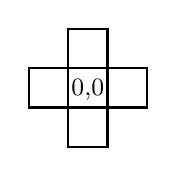
\begin{tikzpicture}
%\draw[step=0.5cm,lightgray,very thin] (0.5,0.5) grid (2,2);
\node at (1.25,1.22) {\textnormal{\small{0,0}}};
\draw[thick] (1,1) rectangle (1.5,1.5);
\draw[thick] (1.5,1) rectangle (2,1.5);
\draw[thick] (1,0.5) rectangle (1.5,1);
\draw[thick] (0.5,1) rectangle (1,1.5);
\draw[thick] (1,1.5) rectangle (1.5,2);
\end{tikzpicture}
\end{center}
%
Each dimension is traversed, coalescing consecutive spans
which vary in $m$-dimensions into coalesced spans which vary in
$m+1$-dimensions. In this example, the $0$-dimensional spans
 become $1$-dimensional spans (rows/columns):
%
\begin{align*}
\begin{array}{cc}
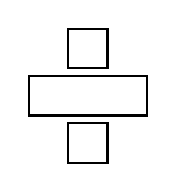
\begin{tikzpicture}
%\draw[step=0.5cm,lightgray,very thin] (0.5,0.5) grid (2,2);
%\node at (1.25,1.22) {\textnormal{\small{0,0}}};
\draw[thick] (0.5,1) rectangle (2,1.5);
\draw[thick] (1,0.40) rectangle (1.5,0.90);
\draw[thick] (1,1.60) rectangle (1.5,2.10);
\end{tikzpicture}
\qquad
&
\qquad
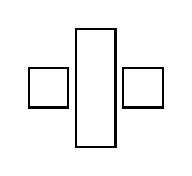
\begin{tikzpicture}
%\draw[step=0.5cm,lightgray,very thin] (0.5,0.5) grid (2,2);
%\node at (1.25,1.22) {\textnormal{\small{0,0}}};
\draw[thick] (1.6,1) rectangle (2.1,1.5);
\draw[thick] (0.4,1) rectangle (0.9,1.5);
\draw[thick] (1,0.5) rectangle (1.5,2);
\end{tikzpicture}
\\
\textit{dimension 1} \qquad & \qquad \textit{dimension 2}
\end{array}
\end{align*}
%
Any spans that are contained with any other span are deleted,
leaving a minimal set of spans (which may overlap, but none of which
fully contains another).
\begin{center}
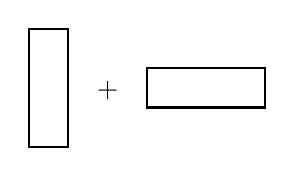
\begin{tikzpicture}
%\node at (1.25,1.22) {\textnormal{\small{0,0}}};
\draw[thick] (1,0.5) rectangle (1.5,2);
\node at (2,1.22) {+};
\draw[thick] (2.5,1) rectangle (4,1.5);
%\node at (2.75,1.22) {\textnormal{\small{0,0}}};
\end{tikzpicture}
\end{center}
%
The procedure is then iterated till a fixed point is reached. In this
example this is reached in the first step. These final spans
go on to form the basis of the spatial stencil specification, where
each span is a region product \texttt{*} and multiple spans are
combined with the region sum \texttt{+}.


\paragraph{Span coalescing, formally}

Let $\vect{x}, \vect{y}, \vect{z}$ range over the column vectors of size
$n$ whose values are drawn from $\mathbb{Z}_\top$.
We write $\vect{x}_i$ for the $i$-th value of vector $\vect{x}$ (1
indexed) and $\vect{x}_{i:j}$ for the sub-vector from entry $i$ to
entry $j$ (inclusive).

\begin{definition}[Spans]
  A \emph{span} represents an $n$-dimensional box (\emph{hyper-rectangle}) as
  a pair of $n$-dimensional vectors (represented as a $2 \times n$
  matrix) giving the co-ordinates of the lower-bound vertex (first
  column) and the upper-bound vertex (second column). We use the
  notation $[\vect{x}^L \; \vect{x}^U]$ for such a span to mark out
  the lower and upper bound vectors.
\end{definition}

The algorithm to create contiguous spans, covering the space of
indices, then proceeds as follows.
Firstly, for all $v \in \mathsf{dom}(M)$ then a new map $M'$ is
created where each vector is mapped to the trivial \emph{unit span} is
created by pairing a vector with itself:
%
\begin{align*}
N(v) = \{[\vect{x} \;
  \vect{x}] \mid \vect{x} \in M(v)\}
\end{align*}
%
For our example, this yields:
%%
\begin{align*}
N(\texttt{a}) = \stwo{0}{0}{0}{0} \stwo{1}{0}{1}{0} \stwo{-1}{0}{-1}{0} \stwo{0}{1}{0}{1} \stwo{0}{-1}{0}{-1}
\end{align*}
%%
A fixed point is then compute for the following
procedure \textsf{regions} which, for per variable
in the map, coalesces spans into contiguous regions in
the $n$-dimensional space. That is, we compute
 $(\mu \; \textsf{regions}) N$ where \textsf{regions}
is defined as follows for each variable in the map:
%
\begin{enumerate}

\item Compute all permutations on the column vectors in a span, \ie{},
  $[\vect{x}^L \vect{x}^U] \mapsto [\pi\vect{x}^L \, \pi\vect{x}^U]$
for a permutation $\pi$. For each permutation function $\pi^n_i$
(the $i$-th permutation for vectors of size $n$, we pair the
permutation function with the set of permuted spans so that
the spans can be un-permuted later.
%
\[
P(v) = \bigcup_{i \in n!} (\pi^n_{i} , \; \{[\pi^n_i
\vect{x}^L \; \pi^n_i\vect{x}^U] \, \mid \, [\vect{x}^L \; \vect{x}^U]
\leftarrow N(v)\}
\]
%
For our example, this yields:
%
\begin{align*}
P(\texttt{a}) =
\{&(\pi^2_1, \{ \stwo{0}{0}{0}{0},
\stwo{1}{0}{1}{0},
\stwo{-1}{0}{-1}{0},
\stwo{0}{1}{0}{1},
\stwo{0}{-1}{0}{-1} \})
\\
&(\pi^2_2, \{
 \stwo{0}{0}{0}{0},
 \stwo{0}{1}{0}{1},
 \stwo{0}{-1}{0}{-1},
 \stwo{1}{0}{1}{0},
 \stwo{-1}{0}{-1}{0}\})\}
\end{align*}
%
where $\pi^2_1$ is the identity permutation and $\pi^2_2$ is the
permutation flips the order of the two elements in the column
vectors.

\item Sort each permutation set into an ordered list, based on the ordering:
\begin{equation*}
  \vect{x} \leq \vect{y} =
      \exists i \, . \; \vect{x}_{i,1} \leq \vect{y}_{i,1} \; \wedge \;
        (i = n \vee \vect{x}_{i+1:n} = \vect{y}_{i+1:n})
\end{equation*}
%
This yields:
%%
\begin{align*}
\{&(\pi^2_1, [
\stwo{0}{-1}{0}{-1},
\stwo{-1}{0}{-1}{0},
\stwo{0}{0}{0}{0},
\stwo{1}{0}{1}{0},
\stwo{0}{1}{0}{1}] )
\\
&(\pi^2_2, [
\stwo{0}{-1}{0}{-1},
\stwo{-1}{0}{-1}{0},
\stwo{0}{0}{0}{0},
\stwo{1}{0}{1}{0},
\stwo{0}{1}{0}{1}])\}
\end{align*}
%%
\item Fold each list pairwise by the following partial operation
 $\bullet$ which coalesces contiguous regions:
%
\begin{align*}
& (\vect{x}^L,\vect{x}^U) \bullet (\vect{y}^L,\vect{y}^U) \\
= &
\begin{cases}
(\vect{x}^L, \vect{y}^U) & \vect{x}^U_1 + 1 = \vect{y}^L_1 \; \wedge \;
\vect{x}_{2:n} = \vect{y}_{2:n}) \\
\bot  & \textit{otherwise}
\end{cases}
\end{align*}
For our example, this yields:
%
\begin{align*}
Q(v) = \{&(\pi^2_1, [
\stwo{0}{-1}{0}{-1},
\stwo{-1}{0}{1}{0},
\stwo{0}{1}{0}{1}
]) \\
&(\pi^2_2, [
\stwo{0}{-1}{0}{-1},
\stwo{-1}{0}{1}{0},
\stwo{0}{1}{0}{1}])\}
\end{align*}
%
\item Un-permute and union together, \ie{},
%
\[
U(v) = \bigcup \{[\pi \vect{x}^L, \pi \vect{x}^U]
 \mid [\vect{x}^L, \vect{x}^U] \leftarrow S, (\pi, S) \leftarrow Q(v)\}
\]
Which yields:
%
\begin{align*}
U(\texttt{a}) =
\{\stwo{0}{-1}{0}{-1},
\stwo{-1}{0}{1}{0},
\stwo{0}{1}{0}{1},
\stwo{-1}{0}{-1}{0},
\stwo{0}{-1}{0}{1},
\stwo{1}{0}{1}{0}\}
\end{align*}
%
\item Finally, filter by the region containment predicate $\containedin$, that
  is, if any region is contained within another then remove the
  smaller. The $\containedin$ predicate is defined:
%
\begin{align*}
& (\vect{x}^L, \vect{x}^U) \containedin (\vect{y}^L, \vect{y}^U) = \\
& \vect{y}^L_1 \leq \vect{x}^L_1 \wedge \vect{x}^U_1 \leq \vect{y}^U_1
  \wedge (\vect{x}^L_{2:n}, \vect{x}^U_{2:n}) \containedin
  (\vect{y}^L_{2:n}, \vect{y}^U_{2:n})
\end{align*}
For our example this then yields the final result of:
\begin{align*}
\textsf{regions}(M)
= \{\stwo{-1}{0}{1}{0} \stwo{0}{-1}{0}{1}\}
\end{align*}
since $\stwo{0}{1}{0}{1} \sqsubseteq \stwo{0}{-1}{0}{1}$
and $\stwo{1}{0}{1}{0} \sqsubseteq \stwo{-1}{0}{1}{0}$.
\end{enumerate}
For our example, applying \textsf{regions} again yields the same
result, hence we have reached a fixed point.

\paragraph{Step 4: Convert spans into region AST}

Given the set $\textsf{regions}(M)$ of spans covering the indexing
space, the next step converts these into abstract syntax trees
for the specification language.

For each span $S = [\vect{l} \; \vect{u}]$,
for each dimension, each pair of entries in the lower- and upper-bound
vectors is mapped to a concrete \textit{spec}, as defined by the
$\mathsf{conv}$ function:
%%
\begin{align*}
& \mathsf{conv}_i\; [\vect{l} \; \vect{u}] = \\
& \begin{cases}
%% FWD
 \stenFwd{\vect{u}_i}{i}{}  & \vect{l}_i = 0 \; \wedge \; \vect{u}_i > 0 \\[0.7em]
 \stenFwd{\vect{u}_i}{i}{, \irreflS}  & \vect{l}_i = 1 \; \wedge \; \vect{u}_i > 0 \\[0.7em]
%% BWD
 \stenBwd{|\vect{l}_i|}{i}{}  & \vect{l}_i < 0 \; \wedge \; \vect{u}_i = 0 \\[0.7em]
\stenBwd{|\vect{l}_i|}{i}{, \irreflS} & \vect{l}_i < 0 \; \wedge \; \vect{u}_i = -1 \\[0.7em]
%% CEN
 \stenCen{\vect{u}_i}{i}{}  &\vect{l}_i < 0 \; \wedge \; \vect{u}_i > 0
 \; \\
 & \qquad\quad \wedge \; |\vect{l}_i| = \vect{u}_i \\[0.7em]
 \stenBwd{|\vect{l}_i|}{i}{} & \vect{l}_i < 0 \; \wedge \; \vect{u}_i >
 0 \\
\quad \texttt{+} \; \stenFwd{\vect{u}_i}{i}{}  & \qquad\quad \wedge \; |\vect{l}_i| \neq \vect{u}_i \\[0.7em]
% ABSOLUTE REP
 \epsilon & \vect{l}_i = \infty \; \vee \; \vect{u}_i
 = \infty \\[0.7em]
% BOUND
 \texttt{atMost}, \stenFwd{\vect{u}_i}{i}{} & \vect{l}_i > 1 \\[0.7em]
 \texttt{atMost}, \stenBwd{|\vect{l}_i|}{i}{} \quad & \vect{l}_i < (-1) \\[0.7em]
  \end{cases}
\end{align*}
%%
The first two cases map to \texttt{forward} stencils since the lower
bound is $0$ or $1$, with the depth determined by the upper bound of
the span. If the lower bound is $1$, then the
$0$-offset point is missing so the specification is given an
\texttt{irreflexive} modifier. The second two cases are similar for
\texttt{backward} but now the depth of the region is determined by the
absolute of the lower bound. In the fifth-case, when the lower bound
is negative and the upper bound is positive and they have the same
magnitude, then a \texttt{centered} region is constructed with
the depth as the common magnitude. If the magnitudes are not the same
(sixth case) then separated \texttt{forward} and \texttt{backward}
regions are summed, with their corresponding depths.

In the case where either bound is $\infty$, representing a non
neighbourhood index, then a simple \texttt{irreflexive} specification
is given with no regions, indicating that there is not even reflexive
0-offset access in this dimension.

Finally in the last two cases, if the lower bound is greater than 1
(which implies the upper bound is greater than 1 too) then
this represents a region that is not at the origin (or next to) the
origin and thus cannot be represented in the specification language.
Thus, an upper bound is instead returned showing the maximum extent
of the region. The last case is the dual, when the lower bound is less
than $-1$, giving an upper bound on a \texttt{backward} specification.

\begin{lemma}
$\mathsf{conv}_i$ is total given the precondition that the lower
bound of the input span is less than or equal to its upper bound.
\end{lemma}

\section{Evaluation}
\label{sec:evaluation}
We evaluated our stencil language on a corpus of scientific code. We first give an overview of the corpus itself before presenting our results.

\subsection{Software Corpus}
\begin{figure}
\begin{tabular}{|l|l|l|l|}
\hline
Package       & Files & Lines of code & Files analysed \\
\hline
UM            & \umFiles & \umLoC & \umparseOk  \\
E3MG          & \ethreemgeaFiles   & \ethreemgeaLoC & \ethreemgeaparseOk  \\
BLAS          & \blasFiles   & \blasLoC & \blasparseOk        \\
Hybrid4       & \hybridfourFiles    & \hybridfourLoC & \hybridfourparseOk         \\
GEOS-Chem     & \geoschemFiles   & \geoschemLoC & \geoschemparseOk       \\
Navier        & \navierFiles     & \navierLoC & \navierparseOk           \\
CP            & \computationalphysicstwoFiles    & \computationalphysicstwoLoC & \computationalphysicstwoparseOk           \\
\hline
\textbf{Total}& \overallFiles  & \overallLoC   & \overallparseOk  \\
\hline
\end{tabular}
\caption{Summary of software packages used for evaluation\label{fig:corpus}}
\end{figure}

Figure \ref{fig:corpus} shows summary statistics of the software packages used in our evaluation, all of which are written in Fortran 90 or Fortran 77. In total we analysed 1.1 million lines of code from 7 packages. The ``Files analysed'' column shows the number of files in each corpus that we were able to analyse with Camfort. The most common reasons for Camfort rejecting a file were either use of a C-preprocessor, or illegal use of language features from a more modern Fortran variant.

\textbf{The Unified Model}\footnote{\url{http://www.metoffice.gov.uk/research/modelling-systems/unified-model}} is a weather forecasting and climate modelling tool developed by the Met Office in the United Kingdom. It is used by research organisations and meteorological services around the world. We use the development branch (trunk) of the model. The Met Office runs a comprehensive code quality system incorporating dedicated committers (we counted 11) for particular parts of the model. We counted 120 additional contributors whose submissions are reviewed and tested before being accepted into the code base.

% e3mg-ea
\textbf{E3MG} (An Energy-Environment-Economy (E3) Model at the Global Level) is a macroeconomic model used for assessment of environmental policy~\cite{RePEc:aen:journl:2006se-a12}. This model was developed by Cambridge Econometrics, an independent consultancy company.

\textbf{BLAS} (Basic Linear Algebra Subprograms)\footnote{\url{http://www.netlib.org/blas/}} provides efficient and portable routines for vector and matrix operations. These routines feature in many other libraries (including LAPACK). We used version 3.6.0.

\textbf{Hybrid4} is a vegetation and biomass model for simulating carbon, water and nitrogen flows~\cite{GBC:GBC635}.

\textbf{GEOS-Chem}\footnote{\url{http://acmg.seas.harvard.edu/geos/}} is a three-dimensional model of tropospheric chemistry developed at Harvard and used by approximately 70 universities and research institutions world-wide. We examined version 10-01.

\textbf{Navier} is an implementation of a Navier-Stokes fluid dynamics computation~\cite{griebel1997numerical}.

\textbf{CP} consists of the example code from the book ``Computational Physics''~\cite{nicholas2006computational} introducing numerical techniques and their application to modern physics problems such as fields, waves, statistical mechanics and quantum mechanics.


% atLeast: number of stencils with an atLeast modifier
% atMost: number of stencils with an atMost modifier
% boundedBoth: number of stencils with both atLeast and atMost modifier
%% atLeast == atMost == boundedBoth - whenever we infer one we infer the other but users might write just one

% backward: number of backward stencils
% forward: number of forward stencils
% centereed: number of centered stencils

% justReflexive: number of only reflexive stencils
% irreflexive: number of irreflexive stencils
% readOnce: number of readOnce stencils

% depthX: number of stencils with depth X
% dimsX: number of stencils with dimensions=X (check this!)

% lexFailed: number of files we failed to lex
% parseFailed: number of files we failed to parse
% lexOrParseFailed: number files we failed to lex and parse
% parseOk: number of files parsed successfully
%% lexFailed + parseFailed = lexOrParseFailed
%% lexOrParseFailed + parseOk = number of files in source repo

% tickAssign: number of array subscripts with a LHS which are all neighbour indices or constants
% tickAssignSuccess: number of tickAssign's we generated some specification for
%% tickAssign < tickAssignSuccess

\subsection{Occurrences of stencils}

We first examined how frequently stencil computations occur in our
corpus. We define a \emph{potential} statement as one whose left-hand
side is an array subscript on neighbourhood indices. These statements
are the inputs to Step 2 of the Inference process described
Section~\ref{sec:inference}. Each potential statement for which we
eventually generate some stencil specifications for is also counted as
an \emph{actual} statement.

\begin{figure}
\begin{tabular}{|l|l|l|l|l|}
\hline
Package       & \% potential & \% actual & Total & Total    \\
              & stencils     & stencils  & exact  & bounded \\
\hline
UM            & \umtickAssignPercent & \umtickAssignSuccessPercent & \umnumStencilLines & \umboundedBoth  \\
E3MG          & \ethreemgeatickAssignPercent & \ethreemgeatickAssignSuccessPercent & \ethreemgeanumStencilLines & \ethreemgeaboundedBoth \\
BLAS          & \blastickAssignPercent & \blastickAssignSuccessPercent & \blasnumStencilLines & \blasboundedBoth \\
Hybrid4       & \hybridfourtickAssignPercent & \hybridfourtickAssignPercent & \hybridfournumStencilLines &  \hybridfourboundedBoth\\
GEOS-Chem     & \geoschemtickAssignPercent & \geoschemtickAssignPercent & \geoschemnumStencilLines & \geoschemboundedBoth \\
Navier        & \naviertickAssignPercent & \naviertickAssignPercent & \naviernumStencilLines & \navierboundedBoth \\
CP            & \computationalphysicstwotickAssignPercent & \computationalphysicstwotickAssignSuccessPercent & \computationalphysicstwonumStencilLines & \computationalphysicstwoboundedBoth \\
\hline
\textbf{Total}& \overalltickAssignPercent  & \overalltickAssignSuccessPercent & \overallnumStencilLines & \overallboundedBoth    \\
\hline
\end{tabular}
\caption{Stencil assignment rates\label{fig:tickAssign}}
\end{figure}

The first two columns of Figure \ref{fig:tickAssign} shows the percentage of lines which were
assigned potential and actual stencils.
\anote{Add explanation about why our results are low. Include an example from BLAS of a tickAssign'd statement that is not a stencil}
\anote{Add discussion about the rate of stencils in the code. Comparison with rate of assignment statements would be nice}

If the inference process cannot determine an exact stencil for a statement it will instead produce an upper (\term{atMost}) and lower (\term{atLeast}) bound. The numbers of exact and bounded stencils are shown in columns three and four of Figure \ref{fig:tickAssign}. We can see that our stencil language is capable of precisely specifying the overwhelming majority of stencils. Most of the bounded stencils apply to some form of data copying. For example (taken from E3MG):
\begin{minted}{fortran}
!- stencil atLeast, readOnce, irreflexive(dims=2), (reflexive(dim=1)) :: sfda
!- stencil atMost, readOnce, (forward(depth=8, dim=2))*(reflexive(dim=1)) :: sfdt
ZZ1(I,J) = SFDT(I,J+8)
\end{minted}




\section{Discussion}
\label{sec:discussion}

\subsection{Related work}

Various prior approaches to specifying and verifying the behaviour
of stencils have been based on fine-grained representations of the
code. These essentially duplicate the indexing scheme of a stencil
computation in their specifications.

\citet{kamil2016verified} propose a technique they call
\emph{verified lifting} for mapping low-level, possibly
greatly optimised, stencil computations into a high-level
predicate language using inductive program synthesis.
The aim is that these high-level abstract specifications can
then be translated into high-performance DSLs, easing the
use of high-performance DSLs. Compared to our approach,
their specification language is more fine grained, capturing
the exact indexing pattern of a stencil. For example, the following
is an example post-condition in their language, generated by their
compiler \textsc{stng} from a Fortran stencil computation~\cite [p.3]{kamil2016verified}:
%
\begin{align*}
& \textit{post}(\texttt{a}, \texttt{b}) \equiv \forall \texttt{imin}+1
\leq \texttt{i} \leq \texttt{imax}, \texttt{jmin} \leq \texttt{j} \leq
\texttt{jmax} \\
& \qquad \texttt{a}(\texttt{i},\texttt{j}) =
\texttt{b}(\texttt{i}-1,\texttt{j}) + \texttt{b}(\texttt{i},\texttt{j})
\end{align*}
%
Noticeable, the bounds of the stencil and the exact indexing pattern
are captured. Our approach aims to be much more abstract, to
facilitate human reasoning, and avoid low-level lexical
errors. However, \textsf{stng} specifications are generated, \ie{},
are never written by a programmer, avoiding this
problem. Their inductive program synthesis approach allows
specifications to extracted even from optimised and unrolled code. For
example, the above post condition is generated from the code~\cite [p.3]{kamil2016verified}:
%
\begin{minted}{fortran}
do j=jmin, jmax
    t = b(imin, j)
    do i=imin+1,imax
        q = b(i, j)
        a(i, j) = q + t
        t = q
    end do
end do
\end{minted}
%
Thus, \textsc{stng} can understand cross-loop data-dependencies
in order to assign the above post-condition. CamFort is not currently
able to ascribe a specification in the above case as the use of
\texttt{t} on line 5 maps only to the definition on line 2, and no on
line 6. Extending our approach to follow loop-carried dependencies is
future work. An alternate approach for us would be to build ontop of
the work of Kamil~\emph{et al.} by inferring our specifications from
\textsc{stng} (as an intermediate step).

In an alternate approach,~\citet{abe2013model}

There are many DSLs for stencil comptuation aimed at either
performance or verification, or both. Many elimiante out-of-bounds
errors, \eg{},~\cite{DBLP:journals/corr/abs-1109-0777}.


\bibliography{references}


\onecolumn
\appendix

\section{Correctness}


\begin{theorem}[Soundness]
\[
S \equiv T
\quad
\Rightarrow
\quad
\interp{S} \equiv \interp{T}
\]
\end{theorem}

\begin{proof}
We will prove different cases given in Figure~\ref{fig:equations} with respect
to the model given in Section~\ref{sec:semantics}.

\begin{description}
  \item[\textsc{Case F \texttt{+} F}:]
    \begin{align*}
      & \; \interp{\stenFwdS{a}{d} \; \texttt{+} \; \stenFwdS{b}{d}}_{n} \\
      \equiv & \; \interp{\stenFwdS{a}{d}}_{n} \; \cup \; \interp{\stenFwdS{b}{d}}_{n} \\
      \equiv & \; \{i\singleEntry{d}{n} \mid i \in \{0, \ldots, a\} \} \; \cup \;
                  \{i\singleEntry{d}{n} \mid i \in \{0, \ldots, b\} \} \\
      \equiv & \; \{i\singleEntry{d}{n} \mid i \in \{0, \ldots, a\}
                    \vee i \in \{0, \ldots, b\} \} \\
      \equiv & \; \{i\singleEntry{d}{n} \mid i \in \{0, \ldots, a \max b\} \} \\
      \equiv & \; \interp{\stenFwdS{a \, \max \, b}{d}}_n \\
    \end{align*}
  \item[\textsc{Case C \texttt{+} C}:]
    \begin{align*}
      & \; \interp{\stenCenS{a}{d} \; \texttt{+} \; \stenCenS{b}{d}}_{n} \\
      \equiv & \; \interp{\stenCenS{a}{d}}_{n} \; \cup \; \interp{\stenCenS{b}{d}}_{n} \\
      \equiv & \; \{i\singleEntry{d}{n} \mid i \in \{-a, \ldots, a\} \} \; \cup \;
                  \{i\singleEntry{d}{n} \mid i \in \{-b, \ldots, b\} \} \\
      \equiv & \; \{i\singleEntry{d}{n} \mid i \in \{-a, \ldots, a\}
                    \vee i \in \{-b, \ldots, b\} \} \\
      \equiv & \; \{i\singleEntry{d}{n} \mid i \in \{- (a \max b), \ldots, a \max b\} \} \\
      \equiv & \; \interp{\stenCenS{a \, \max \, b}{d}}_n \\
    \end{align*}
  \item[\textsc{Case B \texttt{+} B}:]
    \begin{align*}
      & \; \interp{\stenBwdS{a}{d} \; \texttt{+} \; \stenBwdS{b}{d}}_{n} \\
      \equiv & \; \interp{\stenBwdS{a}{d}}_{n} \; \cup \; \interp{\stenBwdS{b}{d}}_{n} \\
      \equiv & \; \{i\singleEntry{d}{n} \mid i \in \{-a, \ldots, 0\} \} \; \cup \;
                  \{i\singleEntry{d}{n} \mid i \in \{-b, \ldots, 0\} \} \\
      \equiv & \; \{i\singleEntry{d}{n} \mid i \in \{-a, \ldots, 0\}
                    \vee i \in \{-b, \ldots, 0\} \} \\
      \equiv & \; \{i\singleEntry{d}{n} \mid i \in \{- (a \max b), \ldots, 0\} \} \\
      \equiv & \; \interp{\stenBwdS{a \, \max \, b}{d}}_n \\
    \end{align*}
  \item[\textsc{Case C \texttt{+} F}:]
    \begin{align*}
      & \; \interp{\stenCenS{a}{d} \; \texttt{+} \; \stenFwdS{b}{d}}_{n} \\
      \equiv & \; \interp{\stenCenS{a}{d}}_{n} \; \cup \; \interp{\stenFwdS{b}{d}}_{n} \\
      \equiv & \; \{i\singleEntry{d}{n} \mid i \in \{-a, \ldots, a\} \} \; \cup \;
                  \{i\singleEntry{d}{n} \mid i \in \{0, \ldots, b\} \} \\
      \equiv & \; \{i\singleEntry{d}{n} \mid i \in \{-a, \ldots, a\}
                    \vee i \in \{0, \ldots, b\} \} \\
      \equiv & \; \{i\singleEntry{d}{n} \mid i \in \{-a, \ldots, a\} \} \quad \text{, using }a \geq b \\
      \equiv & \; \interp{\stenCenS{a}{d}}_n \\
    \end{align*}
  \item[\textsc{Case C \texttt{+} B}:]
    \begin{align*}
      & \; \interp{\stenCenS{a}{d} \; \texttt{+} \; \stenBwdS{b}{d}}_{n} \\
      \equiv & \; \interp{\stenCenS{a}{d}}_{n} \; \cup \; \interp{\stenBwdS{b}{d}}_{n} \\
      \equiv & \; \{i\singleEntry{d}{n} \mid i \in \{-a, \ldots, a\} \} \; \cup \;
                  \{i\singleEntry{d}{n} \mid i \in \{-b, \ldots, 0\} \} \\
      \equiv & \; \{i\singleEntry{d}{n} \mid i \in \{-a, \ldots, a\}
                    \vee i \in \{-b, \ldots, 0\} \} \\
      \equiv & \; \{i\singleEntry{d}{n} \mid i \in \{-a, \ldots, a\} \} \quad \text{, using }a \geq b \\
      \equiv & \; \interp{\stenCenS{a}{d}}_n \\
    \end{align*}
  \item[\textsc{Case B \texttt{+} F}:]
    \begin{align*}
      & \; \interp{\stenBwdS{a}{d} \; \texttt{+} \; \stenFwdS{a}{d}}_{n} \\
      \equiv & \; \interp{\stenBwdS{a}{d}}_{n} \; \cup \; \interp{\stenFwdS{a}{d}}_{n} \\
      \equiv & \; \{i\singleEntry{d}{n} \mid i \in \{-a, \ldots, 0\} \} \; \cup \;
                  \{i\singleEntry{d}{n} \mid i \in \{0, \ldots, a\} \} \\
      \equiv & \; \{i\singleEntry{d}{n} \mid i \in \{-a, \ldots, 0\}
                    \vee i \in \{0, \ldots, a\} \} \\
      \equiv & \; \{i\singleEntry{d}{n} \mid i \in \{-a, \ldots, a\} \} \\
      \equiv & \; \interp{\stenCenS{a}{d}}_n \\
    \end{align*}
  \item[\textsc{Case +COMM}:] Follows from commutativity of union of sets.
  \item[\textsc{Case +ASSOC}:] Follows from associativity of union of sets.
  \item[\textsc{Case *COMM}:] $\interp{r_1 \; \texttt{$\ast$} \; r_2}_n =
    \interp{r_1}_n \otimes \interp{r_2}_n$. Hence, $\texttt{$\ast$}$ is
    commutative iff $\otimes$ is commutative. Now let $\interp{r_1}_n$ and
    $\interp{r_2}_n$ be $S$ and $T$ respectively. Then from the definition of
    $\otimes$, we have $S \otimes T = \{ (s \bowtie t)_i \mid i \in
    \{ 1, \ldots, 2^n \}, (s,t) \in S \times T \}$. Then to show
    commutativity of $\otimes$, it is enough to show any row vector of $s
    \bowtie t$ is also a row vector in the matrix $t \bowtie s$ possibly with a
    different row index.

    Now let $\neg$ be a unary operator over logical matricies that revert $1$s
    to $0$s and vice versa. Then we can define pairwise permutation as
    $(t \bowtie s)_i = t \odot b_i + s \odot \neg b_i$. Now since $i$ ranges
    over all bit strings of length $n$, for all $i$ there is a $j$ such that
    $b_j = \neg b_i$. Hence for all $i$,

    \begin{align*}
      (t \bowtie s)_i &= t \odot b_i + s \odot \neg b_i \\
                      &= t \odot \neg b_j + s \odot \neg (\neg b_j) \\
                      &= s \odot \neg b_j + t \odot b_j \\
                      &= (s \bowtie t)_j
    \end{align*}

  \item[\textsc{Case *ASSOC}:]
  \item[\textsc{Case DIST}:]
\end{description}
\end{proof}


\end{document}

%%  LocalWords:  refactoring affine parameterised irreflexive atMost
%%  LocalWords:  centered readOnce atLeast discretisation Equational
%%  LocalWords:  equational disjunction denotational dimensionality
%%  LocalWords:  interprocedural Fortran Camfort preprocessor
%%  LocalWords:  committers
